%%%%%%%%%%%%%%%%%%%%%%%%%%%%%%%%%%%%%%%%%
% Beamer Presentation
% LaTeX Template
% Version 2.0 (10/06/16)
%
% Attention:
% 0. The self-defined font is used, because 'Calibri' is 
% not supported in the latex font packages. 'LuaLatex'
% should be used.
% 1. This template has been generated according to 
% the Power Point template of LUMC in 2016. 
% 2. This is generated purely with images as the 
% background.
% 3. The bullet point color was used purely for personal 
% preference. 
% 4. Any more adding to the template are welcome. 
% 5.In order to use the navigation bar, the title 
% for each section should not be to long. 
% 6.Adding animation is possible. I prefer to add another
% pdf file with:
% \animategraphics[parameters]{1}{fname}{startnum}{endnum}
% 7. This is my first template, the files might be not  
% well organized, sorry for that. 
% 
% Author:
% Shengnan Liu
% sliu729@gmail.com
% Division Medical imaging processing, 
% Leiden University Medical Center
% 
%%%%%%%%%%%%%%%%%%%%%%%%%%%%%%%%%%%%%%%%%
% Modification Log:
% Generated by Shengnan Liu on 21-01-2016
% Cleaned up for further usage on 10-06-2016
%%%%%%%%%%%%%%%%%%%%%%%%%%%%%%%%%%%%%%%%%
\documentclass[aspectratio=169]{beamer}
\beamertemplatenavigationsymbolsempty%
\usepackage{textpos}
\usefonttheme[onlymath]{serif}
\usepackage{amsmath}
\usepackage{bm}
\usepackage{empheq}
\usepackage{eso-pic}
\usepackage{fontspec}
\usepackage{hyperref}
\usepackage{textcomp}
\usepackage{multirow}
\setsansfont{Linux Biolinum O}
%\setmainfont{Gentium}
\usetheme{Rochester}% theme
\usecolortheme{seahorse}
\colorlet{beamer@blendedblue}{green!40!black}
%\setbeamertemplate{navigation symbols}{}
%\setbeamertemplate{footline}[frame number]
\setbeamertemplate{footline}{% hide total number of slides
  \hfill% 
  \usebeamercolor[fg]{page number in head/foot}% 
  \usebeamerfont{page number in head/foot}% 
  \insertframenumber%
  \kern1em\vskip2pt% 
}
\setbeamertemplate{itemize items}[circle]
\hypersetup{
    colorlinks = true,
    urlcolor = cyan
}

% Define color "lightgreen" for highlighting equarions
\definecolor{lightgreen}{HTML}{90EE90}

\addtobeamertemplate{frametitle}{}{%
\begin{textblock*}{100mm}(.80\textwidth,-1.55cm)

\includegraphics[height=1.5cm]{figures/csu-logo.png}
\end{textblock*}}

\title{A Shallow Learning Hadronic Energy Estimator}
\date[today]{\today}
\author{Shih-Kai Lin}
\institute{Colorado State University}
\usepackage{multicol} % 
%\usepackage{animate}  % animation
\usepackage{amsmath,amsfonts,amssymb} % This makes the equations appears better 
\begin{document}
%The title
\begin{frame}
\titlepage
\end{frame}


% Adding note that cannot be seen
\note[itemize]{
\item Good morning everyone. Today I would like to present the work that were submitted to SPIE proceeding photonics west. 
\item point 2
}

% The outline
%\begin{frame}{Outline}
%\tableofcontents
%\end{frame}

\begin{frame}{Some Teaser}
  \centering
  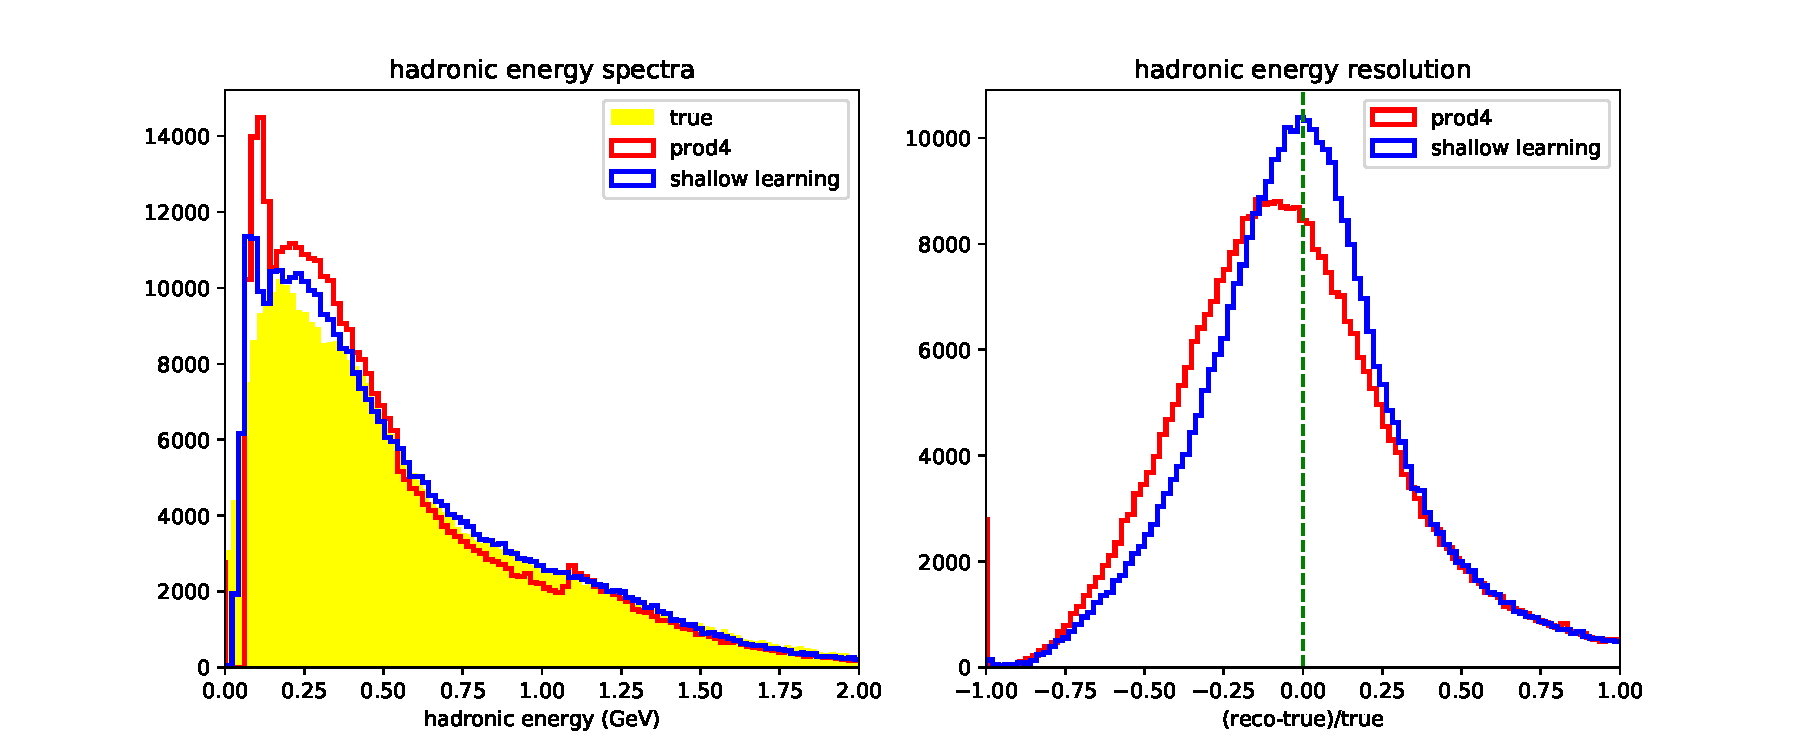
\includegraphics[width=\textwidth]{figures/ehad_spec_res_side_by_side.pdf}
\end{frame}

\begin{frame}{Motivation}
  \begin{itemize}
    \item NOvA has put a lot of effort into PID (classification) with the state-of-the-art machine learning techniques, but not as much in energy reconstruction (regression).
    \begin{itemize}
      \item Except CVN regression (UCI)
    \end{itemize}
    \item Why one more attempt at energy reconstruction besides the current prong-based one (Erica, Michael) and CVN regression?
    \begin{itemize}
      \item It is a natural generalization to the current official spline fit.
      \begin{itemize}
        \item In the sense that it also uses event-level variables to fit a regression function.
      \end{itemize}
      \item It has welcoming mathematical properties and beautiful underlying theory.
      \item The nice mathematical properties are reflected in the results.
      \item Better tools! There are many CVN final state particle scores available at the moment.
    \end{itemize}
  \end{itemize}
\end{frame}

\begin{frame}{Shallow Learning}
  \begin{itemize}
    \item As opposed to deep learning. Some authors use this term in literature.
    \begin{itemize}
      \item I personally like it due to my initials...
    \end{itemize}
    \item Below is why this class of methods is called shallow learning in contrast to deep learning:    
  \end{itemize}
  \centering
  \scriptsize
  \begin{tabular}{c|ccccc}
    \multirow{2}{*}{deep architecture} & \multirow{2}{*}{CNN} & \multirow{2}{*}{$\longrightarrow$} & \multirow{2}{*}{many hidden layers} & \multirow{2}{*}{$\longrightarrow$} & classification    \\
    &&&&&regression\\
    \hline
    \multirow{2}{*}{shallow architecture} & support vector machine & \multirow{2}{*}{$\longrightarrow$} & one hidden layer & \multirow{2}{*}{$\longrightarrow$} & classification\\
    & kernel ridge regression & & (feature map) & & regression\\
  \end{tabular}
  \normalsize
  \begin{itemize}
    \item A cohort of \emph{kernel methods} belongs to shallow architecture, among which the support vector machine was so popular that it almost killed neural network in the early 2000s before CNN took the crown.
    \item I will quickly go through the ideas behind kernel methods to justify the use of them for an energy estimator.
  \end{itemize}
\end{frame}

%\begin{frame}{Ideas behind Kernel Methods -- from the Most Basic}
%\scriptsize
%Linear regression:\\
%Given $N$ training samples, $(\mathbf{x}_i,y_i)$, $i=1,...,N$, where $\mathbf{x}_i$'s $\in\mathbb{R}^\ell$ are predictor variables and $y_i$'s $\in\mathbb{R}$ are target variables of training samples, find a linear function
%\begin{equation}
%  f_\mathbf{w}(\mathbf{x})=\mathbf{w}^T\mathbf{x}
%\end{equation}
%that minimizes the quadratic cost,
%\begin{equation}
%  C(\mathbf{w})=\frac{1}{2}\sum_{i=1}^{N}(y_i-\mathbf{w}^T\mathbf{x}_i)^2
%\end{equation}
%$\mathbf{w}$ that minimizes the cost function is readily found by solving the \emph{normal equation}:
%\begin{equation}
%  \mathbf{X}^T\mathbf{X}\mathbf{w}=\mathbf{X}^T\mathbf{y}
%\end{equation}
%, where $\mathbf{X}$ is the so called \emph{design matrix}, 
%\begin{equation}
%  \mathbf{X}=\begin{pmatrix}\mathbf{x}_1^T \\ \vdots \\ \mathbf{x}_N^T \end{pmatrix}
%\end{equation}
%\end{frame}
%
%\begin{frame}{Ridge Regression and Dual Form}
%\tiny
%Very often, the predictor variables vary in a similar way, known as near collinearity. In such cases, $\mathbf{X}^T\mathbf{X}$ is almost singular, and the resulting $\mathbf{w}$ becomes highly sensitive to variations, leading to overfitting.\\
%Applying Tikhonov regularization leads to ridge regression, namely, minimizing the cost function
%\begin{equation}
%  C(\mathbf{w})=\frac{1}{2}\sum_{i=1}^{N}(y_i-\mathbf{w}^T\mathbf{x}_i)^2+\frac{1}{2}\alpha\Vert\mathbf{w}\Vert^2
%\end{equation}
%with the solution
%\begin{equation}
%  \mathbf{w}=(\mathbf{X}^T\mathbf{X}+\alpha\mathbf{I})^{-1}\mathbf{X}^T\mathbf{y}
%\end{equation}
%\textcolor{blue}{The cost function is convex, which guarantees a global minimum. (Very different from NN case.)}\\
%Note that $\mathbf{w}$ can be rewritten\footnote{See \href{http://stat.wikia.com/wiki/Kernel_Ridge_Regression}{here} for details.} as $\mathbf{w}=\mathbf{X}^T(\mathbf{X}\mathbf{X}^T+\alpha\mathbf{I})^{-1}\mathbf{y}$.\\
%For a test sample $\hat{\mathbf{x}}$, the predicted value $\hat{y}=\mathbf{w}^T\hat{\mathbf{x}}=\hat{\mathbf{x}}^T\mathbf{w}=\hat{\mathbf{x}}^T\mathbf{X}^T(\mathbf{X}\mathbf{X}^T+\alpha\mathbf{I})^{-1}\mathbf{y}$. Now, let $\mathbf{a}=(\mathbf{X}\mathbf{X}^T+\alpha\mathbf{I})^{-1}\mathbf{y}$, we arrive at the \textcolor{red}{\emph{dual form}}:
%\begin{equation}
%  \hat{y}=\sum_{i=1}^{N}a_i\mathbf{x}_i^T\hat{\mathbf{x}}
%\end{equation}
%, i.e., instead of solving for $\mathbf{w}$, we solve for $\mathbf{a}$.
%\end{frame}

\begin{frame}{Ridge Regression}
Given $N$ training samples $(\mathbf{x}_i,y_i)$, where $\mathbf{x}_i\in\mathbb{R}^\ell$ are regressors and $y_i\in\mathbb{R}$ are targets, we want to find a linear function $f_\mathbf{w}(\mathbf{x})=\mathbf{w}^T\mathbf{x}$ that minimizes the squared error loss function with $L_2$ regularization,
\begin{equation}\label{eq:loss}
  L(\mathbf{w})=\underbrace{\sum_{i=1}^{N}(y_i-\mathbf{w}^T\mathbf{x}_i)^2}_\text{squared error}+\underbrace{\alpha\Vert\mathbf{w}\Vert^2}_\text{Tikhonov regularization}
\end{equation}
, where $\alpha$ is a hyperparameter\footnote{A hyperparameter is a parameter whose value is set before the learning process begins.} that controls the degree of overfitting.
\end{frame}

\begin{frame}{Regression Function and Dual Form}
\scriptsize
Solution to \ref{eq:loss} is
\begin{equation}
\mathbf{w}=(\mathbf{X}^T\mathbf{X}+\alpha\mathbf{I})^{-1}\mathbf{X}^T\mathbf{y}
\end{equation}
, where $\mathbf{X}$ is the so called \emph{design matrix}, 
\begin{equation}
  \mathbf{X}=\begin{pmatrix}\mathbf{x}_1^T \\ \vdots \\ \mathbf{x}_N^T \end{pmatrix}
\end{equation}
$\mathbf{w}$ can be rewritten as
\begin{equation}
\mathbf{w}=\mathbf{X}^T(\mathbf{X}\mathbf{X}^T+\alpha\mathbf{I})^{-1}\mathbf{y}
\end{equation}
With this \emph{dual form}, given a test sample $\mathbf{x}_t$, the predicted value is
\begin{equation} \label{eq:sol}
\hat{y}_t=\sum_{i=1}^{N}a_i\mathbf{x}_i^T\mathbf{x}_t
\end{equation}
Here, $\mathbf{a}=(\mathbf{X}\mathbf{X}^T+\alpha\mathbf{I})^{-1}\mathbf{y}$, and $\mathbf{X}\mathbf{X}^T$ is a Gram matrix with elements $[\mathbf{X}\mathbf{X}^T]_{ij}=\mathbf{x}_i^T\mathbf{x}_j$.
\end{frame}

\begin{frame}{Nonlinear Regression with Feature Map}
A second order polynomial can be written as
\begin{equation}
f_\mathbf{w}(x)=w_0+w_1x+w_2x^2=\mathbf{w}^T\bm{\phi}(x)
\end{equation}
With the \emph{feature map} $\bm{\phi}:\mathbb{R}\rightarrow\mathbb{R}^3$, $\bm{\phi}(x)=(1,x,x^2)^T$, nonlinear regression in the \emph{input space} $\mathbb{R}$ is equivalent to linear regression in the \emph{feature space} $\mathbb{R}^3$. \\
Formula obtained with the linear case apply here, as long as $\mathbf{x}$ is replaced by $\bm{\phi}(\mathbf{x})$.
\end{frame}

\begin{frame}{Kernel Trick}
\begin{itemize}
  \item Note that in the solution formula \ref{eq:sol}, every occurrence of a regressor $\mathbf{x}$ is accompanied by another regressor $\mathbf{x}'$ in the form of an inner product of the two.
  \item In the nonlinear case, it's $\bm{\phi}(\mathbf{x})^T\bm{\phi}(\mathbf{x}')$.
  \begin{itemize}
    \item Dimensionality of range of $\bm{\phi}$ becomes implicit and not important anymore.
  \end{itemize}
  \item If we can find a kernel function $k:\mathbb{R}^\ell\times\mathbb{R}^\ell\rightarrow\mathbb{R}$ such that $k(\mathbf{x},\mathbf{x}')=\bm{\phi}(\mathbf{x})^T\bm{\phi}(\mathbf{x}')$, $\forall\mathbf{x},\mathbf{x}'\in\mathbb{R}^\ell$, then we can obtain the solution without actually performing the feature map, which is computationally heavy and sometimes even impossible (ex. infinite-dimensional feature space).
  \item Note that given a kernel the feature map and feature space are not unique.
\end{itemize}
\end{frame}

\begin{frame}{The RBF (Gaussian) Kernel}
\footnotesize
One of the most commonly used kernels is the radial basis function (RBF), or Gaussian kernel:
\begin{equation}
  k(\mathbf{x},\mathbf{x}')=e^{-\gamma\Vert\mathbf{x}-\mathbf{x}'\Vert^2}
\end{equation}
For $\ell=1$, a heuristic feature map of the RBF kernel is
\begin{equation}
  \bm{\phi}(x)=\underbrace{e^{-\gamma x^2}}_\text{local}\underbrace{\left(1,\sqrt{\frac{2\gamma}{1!}}x,\sqrt{\frac{(2\gamma)^2}{2!}}x^2,\dots\right)^T}_\text{polynomial of all orders}
\end{equation}
, where we can see that the feature map of the RBF kernel is like local fit to polynomials of all orders.
\begin{itemize}
  \item The RBF kernel works so well in many cases that it is usually one of the default kernels to try out.
  \begin{itemize}
    \scriptsize
    \item I will use this kernel throughout the study.
  \end{itemize}
    \item The hyperparameter $\gamma$ controls how far the effect of a training sample can reach.
\end{itemize}
\end{frame}

\begin{frame}{Representer Theorem and Kernel Ridge Regression}
The solution function in the nonlinear problem to minimize a class of loss functions, including the squared loss with $L_2$ penalty, is
\begin{empheq}[box=\colorbox{lightgreen}]{equation}
  f(\mathbf{x})=\sum_{i=1}^{N}a_ik(\mathbf{x}_i,\mathbf{x})
\end{empheq}
, where $\mathbf{a}=(\mathbf{K}+\alpha\mathbf{I})^{-1}\mathbf{y}$ and $K_{ij}=k(\mathbf{x}_i,\mathbf{x}_j)$.
\begin{itemize}
  \item Clearly a generalization to eq. \ref{eq:sol}.
  \item Ridge regression with kernel trick is the \textcolor{blue}{kernel ridge regression (KRR)}, one of the few machine learning algorithms with a closed form solution.
  \item I have tried support vector regression (SVR) as well. Since KRR works better, I will only show results from KRR.
\end{itemize}
\end{frame}

\begin{frame}{Features of Kernel Methods}
  \begin{itemize}
    \item Nonparametric model
    \begin{itemize}
      \item Number of parameters grows with number of training samples.
      \item In this case, it's the $\mathbf{a}$ vector.
    \end{itemize}
    \item Unlike the \emph{binned} spline fit, this is an \emph{unbinned} fit.
    \item Positive definite kernels\footnote{Most commonly used kernels belong to this class, including RBF, but not sigmoid.} make the loss function convex. Therefore, a global minimum is guaranteed.
    \begin{itemize}
      \item Very different from neural networks.
    \end{itemize}
    \item Functions drawn from the RBF kernel are \emph{very smooth}.
    \begin{itemize}
      \item No more kinks in the regression curve/surface/hypersurface.
    \end{itemize}
    \item Including more variables is a no-brainer.
    \begin{itemize}
      \item How to design a regression surface embedded in 3D after all? More dimension?
      \item Opens up ``feature engineering".
    \end{itemize}
  \end{itemize}
\end{frame}

\begin{frame}{Hands-on!}
\small
Time to get hands dirty:
\begin{itemize}
  \item datasets\\
  \nolinkurl{prod_caf_R17-11-14-prod4reco.d_nd_genie_nonswap_fhc_nova_v08_period3_v1}
  \item cuts\\
  \nolinkurl{kNumuCutND2018 && kIsNumuCC}
  \item weights
  \begin{itemize}
    \scriptsize
    \item No weight for the proof of concept rounds
    \item For the newest results, \nolinkurl{kXSecCVWgt2018 * kPPFXFluxCVWgt}
  \end{itemize}
  \item variables\\
  regressor
  \begin{itemize}
    \scriptsize
    \item \nolinkurl{kNumuHadVisE} for first attempts
    \item later add CVN particle final state scores for $p$, $n$, $\pi^0$, $\pi^{\pm}$, and number of prongs
  \end{itemize}
  target\\
  \begin{itemize}
    \scriptsize
    \item always \nolinkurl{kTrueE} (true neutrino energy) - \nolinkurl{kMuE} (prod4 reco muon energy)
  \end{itemize}
\end{itemize}
\end{frame}

\begin{frame}{1D regressor ($E_{vishad}$), 0.5\% total statistics}
\centering
\includegraphics[width=\textwidth]{figures/{prod4_krr_side_by_side_a0.5g0.5step200offset0}.pdf}
\end{frame}

\end{document}